% !TeX root = ../main.tex

\parindent=0pt
In questo capitolo viene analizzato il processo di sviluppo tipico per le applicazioni mobile al fine di porre le basi per la progettazione dello stesso processo di sviluppo applicando pratiche e tecniche DevOps di automazione. Lo scopo di questa fase iniziale di progetto è quindi la definizione di tutti i principali task e sotto-task necessari allo sviluppo di applicazioni mobile, dalla scrittura del codice sorgente al rilascio sui marketplace delle relative piattaforme target, le quali sono Android e iOS.

\begin{figure}[H]
\centering
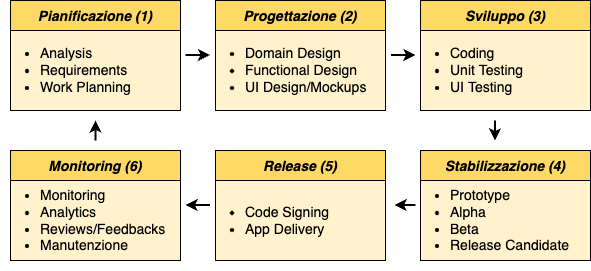
\includegraphics[width=0.75\textwidth]{img/tesi-2-Page-9.drawio.png}
\caption{Ciclo di vita di sviluppo tipico delle applicazioni mobile}
\end{figure}

Il processo di sviluppo delle applicazioni mobile è simile a quello di qualsiasi altra tipologia di applicazione: in questo caso l'obiettivo è distribuire l'applicazione, dando la possibilità all'utente di installarla sul proprio dispositivo, mentre tipicamente nei processi di altre tipologie di applicazioni l'obiettivo è quello di mettere in esecuzione l'applicazione in un ambiente target accessibile all'utente.

\section{Pianificazione}
In questa prima fase del processo di sviluppo si formalizzano i requisiti, funzionali e non funzionali, che devono essere soddisfatti dalla applicazione per ottenere l'approvazione del committente e si pianifica il lavoro per le successive fasi in termini di task, risorse e tempo.\\
Tramite la definizione di casi d'uso si rappresentano le interazioni tra il sistema e dei ruoli (attori in UML\footnote{Unified Modeling Language}) necessarie al raggiungimento di un obiettivo. Questi casi d'uso sono dunque dei possibili scenari dove il sistema riceve delle richieste esterne, come l'input dell'utente, e risponde ad esso.
Dopo aver acquisito un numero appropriato di casi d'uso e attori è molto più semplice iniziare a progettare una applicazione. Lo sviluppo può quindi concentrarsi su come creare l'applicazione anziché sulla sua definizione o la sua funzione.

\section{Progettazione}
La fase di progettazione della applicazione è composta da un insieme di sottotask tra cui la modellazione del dominio applicativo, la scelta della architettura da utilizzare e la prototipazione dell'esperienza utente e dell'interfaccia grafica (UX/UI).\\
Tipicamente la progettazione UX/UI viene svolta tramite l'ausilio di mockup per definire prima come l'utente intende utilizzare l'applicazione (esperienza) e poi aspetti grafici come colori, font e icone (interfaccia).

\section{Sviluppo}
Una volta progettata l'applicazione è possibile partire con la fase di sviluppo. Solitamente l'obiettivo è far iniziare la fase di sviluppo il prima possibile in modo da sviluppare un prototipo funzionante ed ottenere la validazione da parte del committente, la quale è l'obiettivo principale della fase successiva.

\section{Stabilizzazione}
La stabilizzazione consiste nella risoluzione di problemi sia a livello funzionale che a livello di usabilità e di prestazioni al fine di ottenere una versione di applicazione pronta da distribuire. Questa parte del ciclo di sviluppo dovrebbe iniziare il più presto possibile in modo da individuare e risolvere i problemi prima che diventino un costo. Tipicamente per qualsiasi applicazione, anche non specifica per i dispositivi mobile, sono previste le seguenti sottofasi del processo di stabilizzazione\cite{sdlf}:
\begin{itemize}
    \item \textit{Prototype} - L'applicazione include soltanto alcune delle funzionalità principali e sono presenti bug maggiori. In questa fase il focus è sulla singola funzionalità implementata fornita dal prototipo per il testing.
    \item \textit{Alpha} - Tutte le principali funzionalità sono completate e devono essere testate.
    \item \textit{Beta} - Gran parte delle funzionalità, sia principali che ausiliarie, sono state completate e i bug maggiori sono stati risolti.
    \item \textit{Release Candidate} - Tutte le funzionalità sono state completate e testate, ma potrebbero essere presenti ancora bug minori.
\end{itemize}

\subsection{Alpha}
La prima versione funzionante di una applicazione è detta alpha ed è utilizzata per il testing interno di specifiche funzionalità. Questo significa che può presentare anche bug o funzionalità mancanti ma almeno deve contenere le funzionalità che devono essere testate per quella specifica versione alpha. \\
Solitamente prima della release di una applicazione, anche se in fase di testing, è necessario attendere la sua approvazione da parte del gestore del servizio. Il processo di approvazione pre-release è detto \textit{App Review}. Nel caso del testing interno è possibile distribuire la applicazione ad un insieme ristretto di tester.\\
Continuando con i rilasci di versioni alpha vengono aggiunte nuove funzionalità e/o risolti eventuali bug: quando la versione è considerata pronta viene eseguita una sua promozione. Con promozione si intende in questo caso il rilascio di una versione alpha in versione beta.

\subsection{Beta}
A questo punto del processo di sviluppo la applicazione è considerata completa a tutti gli effetti a meno di bug e/o problemi di stabilità. La versione beta rappresenta dunque la prima versione della applicazione resa disponibile ai tester esterni, ovvero quegli utenti che non hanno partecipato alle fasi di sviluppo e che svolgono il ruolo di validazione delle funzionalità. Si distinguono due tipologie di beta testing:
\begin{itemize}
    \item \textit{Aperto} - La applicazione è rilasciata per la fase di testing esterno permettendo l'accesso a qualsiasi utente con account da beta tester. Nel caso di Android per poter testare una applicazione in versione beta aperta è necessario disporre di un account Google Developer.
    \item \textit{Chiuso} - L'accesso alla applicazione di test è limitato ad un insieme ristretto di tester, tipicamente gestiti tramite mailing list o link di condivisione.
\end{itemize}
Dopo aver ottenuto la validazione da parte dei tester, la quale potrebbe richiedere più iterazioni di sviluppo e rilascio di versioni alpha-beta, anche per la versione beta si effettua la promozione, rilasciando la applicazione in produzione.


\section{Release}
Dopo che la applicazione è stata stabilizzata è possibile procedere con la distribuzione. In questa fase l'applicazione viene prima firmata digitalmente utilizzando un certificato protetto da chiave privata e poi pubblicata sullo specifico marketplace della piattaforma target.


\section{Monitoraggio}
La fase di monitoraggio (e manutenzione) è quella più lunga e dispendiosa in termini di tempo e risorse. Per le applicazioni mobile esistono alcune situazioni che rendono il monitoraggio più complesso rispetto ad altre tipologie di applicazioni come ad esempio le web app. Bisogna infatti considerare che\cite{mamonitoring}:
\begin{itemize}
    \item le applicazioni mobile eseguono su una vasta gamma di dispositivi con caratteristiche diverse e può essere quindi difficile ottenere una chiara visibilità delle prestazioni lato client;
    \item se gli utenti riscontrano un problema, mentre una patch per applicazioni web può essere distribuita quasi all'istante, la distribuzione degli aggiornamenti delle applicazioni mobile richiede tempo e l'attivazione da parte degli utenti per scaricarli.
\end{itemize}
Per effettuare un monitoraggio efficace è necessario misurare e controllare continuamente le performance della applicazione mobile, il comportamento dell'utente e gli errori che essi riscontrano. Alcuni esempi di metriche fondamentali sono: tempo di avvio della applicazione, network performance, utilizzo delle risorse (CPU, disco e memoria) e metriche custom derivanti dalle azioni dell'utente.